\section{Specifica della componente Service}
Questa componente è incaricata elaborare le richieste arrivate dai controller restituendo i dati richiesti e quando necessario interroga la componente model per ottenere i dati dal database.
Tale componente è composta dalle classi:
\begin{itemize}
	\item \texttt{com.sirius.sequenziatore.server.service.SignUpService}
	\item \texttt{com.sirius.sequenziatore.server.service.LoginService}
	\item \texttt{com.sirius.sequenziatore.server.service.StepInfoService}
	\item \texttt{com.sirius.sequenziatore.server.service.ProcessInfoService}
	\item \texttt{com.sirius.sequenziatore.server.service.StepService}
	\item \texttt{com.sirius.sequenziatore.server.service.ProcessService}
	\item \texttt{com.sirius.sequenziatore.server.service.ApproveStepService}
	\item \texttt{com.sirius.sequenziatore.server.service.UserStepService}
	\item \texttt{com.sirius.sequenziatore.server.service.UserProcessService}
	\item \texttt{com.sirius.sequenziatore.server.service.ReportService}
\end{itemize}
Qui di seguito verranno ora analizzate le singole classi di tale componente, tali classi sono annotate con @Service, in modo da essere riconosciute in modo corretto da Spring.
\subsection{Package com.sirius.sequenziatore.server.service}
\begin{figure}[H] \centering 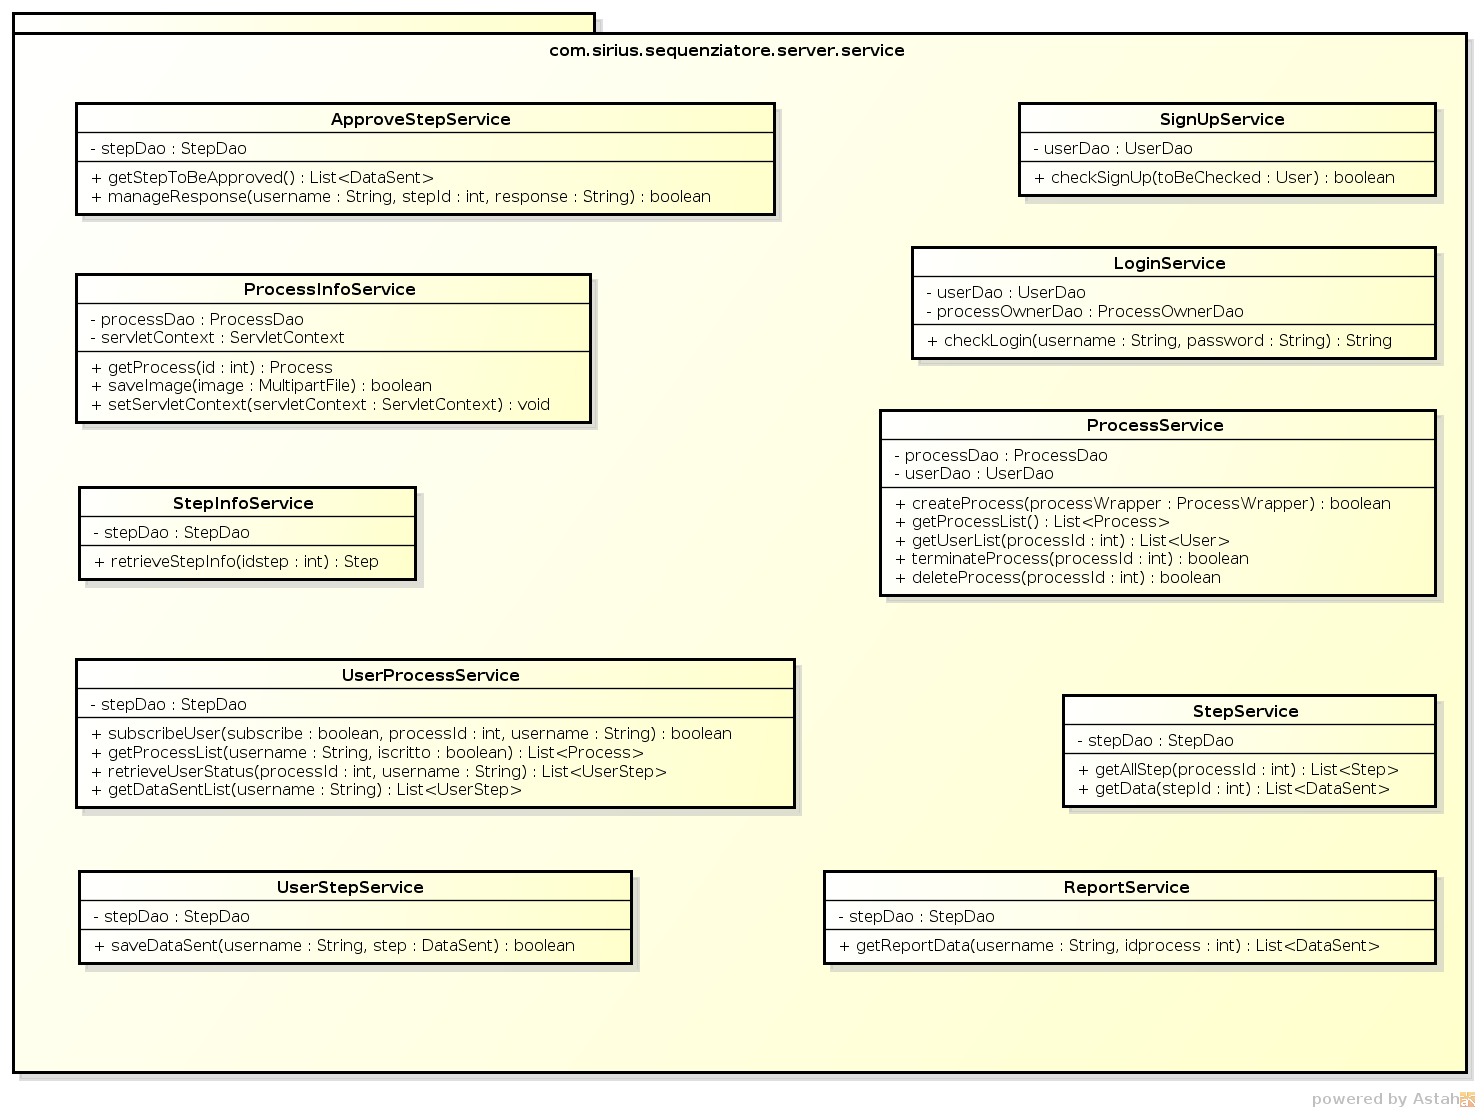
\includegraphics[width=%
\textwidth]
{./classi/server/service.png} \caption{Diagramma package - \texttt{com.sirius.sequenziatore.server.service}}
\end{figure}
\paragraph{SignUpService}%--------------------------------------------------------%
\
\begin{figure}[H] \centering
\includegraphics[trim=0cm 0.8cm 0cm 0cm,clip=true,scale=0.75]%
{./classi/server/signupservice.png} \caption{Diagramma classe - \texttt{SignUpService}}
\end{figure}
\begin{itemize}
	\item \textbf{Descrizione: } Questa classe dovrà elaborare tutte le richieste di registrazione al sistema ricevute dal client, sarà incaricata di inserire i dati nel database.
	\item \textbf{Relazioni con altri componenti: }
	La classe utilizzerà le seguenti classi:
	\begin{itemize}
		\item \texttt{com.sirius.sequenziatore.server.model.UserDao;}
		\item \texttt{com.sirius.sequenziatore.server.model.User;}
	\end{itemize}
	\item \textbf{Attributi:}\begin{itemize}
					\item \texttt{-UserDao userDao}:\\
					oggetto usato per inserire il nuovo utente nel database;
	\end{itemize}
	\item \textbf{Metodi: }\begin{itemize}
					\item \texttt{+boolean checkSignUp(User toBeChecked)}:\\
					 questo metodo deve inserire nel database il nuovo utente ricevuto, e ritornare l' esito di tale operazione al controller;
				\end{itemize}
\end{itemize}
\paragraph{ApproveStepService}%--------------------------------------------------------%
\
\begin{figure}[H] \centering
\includegraphics[trim=0cm 0.8cm 0cm 0cm,clip=true,scale=0.75]%
{./classi/server/approvestepservice.png} \caption{Diagramma classe - \texttt{ApproveStepService}}
\end{figure}
\begin{itemize}
	\item \textbf{Descrizione: } Questa classe dovrà elaborare tutti gli esiti della moderazione dei passi del processowner quindi accettare o rifiutare i passi in attesa di approvazione.
	\item \textbf{Relazioni con altri componenti: }
	La classe utilizzerà le seguenti classi:
	\begin{itemize}
		\item \texttt{com.sirius.sequenziatore.server.model.StepDao;}
		\item \texttt{com.sirius.sequenziatore.server.model.DataSent;}
	\end{itemize}
	\item \textbf{Attributi:}\begin{itemize}
					\item \texttt{-StepDao stepDao}:\\
					oggetto usato per modificare i passi nel database secondo l' esito del process owner;
	\end{itemize}
	\item \textbf{Metodi: }\begin{itemize}
					\item \texttt{+List<DataSent> getStepToBeApproved()}:\\
					questo metodo ritorna una lista di passi che sono in attesa di approvazione, dopo averla ottenuta dal database tramite stepDao;
					\item \texttt{+boolean manageResponse(String username,int stepId,String response):}\\
					questo metodo permette di gestire l' esito della moderazione del process owner per un dato passo di un dato utente, in \texttt{response} sarà contenuto tale esito che sarà \textit{APPROVED} o \textit{REJECTED} e poi andrà a modificare il passo nel database tramite stepDao;
				\end{itemize}
\end{itemize}
\paragraph{ProcessInfoService}%--------------------------------------------------------%
\
\begin{figure}[H] \centering
\includegraphics[trim=0cm 0.8cm 0cm 0cm,clip=true,scale=0.75]%
{./classi/server/processinfoservice.png} \caption{Diagramma classe - \texttt{ProcessInfoService}}
\end{figure}
\begin{itemize}
	\item \textbf{Descrizione: } Questa classe dovrà elaborare le varie richieste di tutti gli utenti per quanto riguarda le informazioni generali di un processo, quindi la sua struttura e permette il salvataggio di immagini;
	\item \textbf{Relazioni con altri componenti: }
	La classe utilizzerà le seguenti classi:
	\begin{itemize}
		\item \texttt{com.sirius.sequenziatore.server.model.ProcessDao;}
		\item \texttt{com.sirius.sequenziatore.server.model.Process;}
	\end{itemize}
	\item \textbf{Attributi:}\begin{itemize}
					\item \texttt{-ProcessDao processDao}:\\
					oggetto usato per modificare i passi nel database secondo l' esito del process owner;
	\end{itemize}
	\item \textbf{Metodi: }\begin{itemize}
					\item \texttt{+Process getProcess(int id)}:\\
					questo metodo ritorna la struttura del processo richiesto;
					\item \texttt{+boolean saveImage(MultipartFile image):}\\
					questo metodo permette il salvataggio delle immagini del processo;
					\item \texttt{+void setServletContext(ServletContext servletContext):}
					questo metodo serve per settare la servletContext;
				\end{itemize}
\end{itemize}
\paragraph{StepInfoService}%--------------------------------------------------------%
\
\begin{figure}[H] \centering
\includegraphics[trim=0cm 0.8cm 0cm 0cm,clip=true,scale=0.75]%
{./classi/server/stepinfoservice.png} \caption{Diagramma classe - \texttt{StepInfoService}}
\end{figure}
\begin{itemize}
	\item \textbf{Descrizione: } Questa classe dovrà elaborare le varie richieste di tutti gli utenti per quanto riguarda le informazioni generali di un passo, quindi la sua struttura;
	\item \textbf{Relazioni con altri componenti:}
	La classe utilizzerà le seguenti classi:
	\begin{itemize}
		\item \texttt{com.sirius.sequenziatore.server.model.StepDao;}
		\item \texttt{com.sirius.sequenziatore.server.model.Step;}
	\end{itemize}
	\item \textbf{Attributi:}\begin{itemize}
					\item \texttt{-StepDao stepDao}:\\
					oggetto usato per ottenere i dati di un passo;
	\end{itemize}
	\item \textbf{Metodi: }\begin{itemize}
					\item \texttt{+Step retrieveStep(int idStep)}:\\
					questo metodo ritorna la struttura del passo richiesto;
				\end{itemize}
\end{itemize}
\paragraph{LoginService}%--------------------------------------------------------%
\
\begin{figure}[H] \centering
\includegraphics[trim=0cm 0.8cm 0cm 0cm,clip=true,scale=0.75]%
{./classi/server/loginservice.png} \caption{Diagramma classe - \texttt{LoginService}}
\end{figure}
\begin{itemize}
	\item \textbf{Descrizione: } Questa classe elaborerà le richieste di login 
	\item \textbf{Relazioni con altri componenti: }
	La classe utilizzerà le seguenti classi:
	\begin{itemize}
		\item \texttt{com.sirius.sequenziatore.server.model.UserDao;}
		\item \texttt{com.sirius.sequenziatore.server.model.ProcessOwnerDao;}
	\end{itemize}
	\item \textbf{Attributi:}\begin{itemize}
					\item \texttt{-UserDao userDao}:\\
					oggetto usato per ottenere i dati di un utente;
					\item \texttt{-ProcessOwnerDao processOwnerDao}:\\
					oggetto usato per ottenere i dati di un processowner;
	\end{itemize}
	\item \textbf{Metodi: }\begin{itemize}
					\item \texttt{+String checkLogin(String username,String password)}:\\
					questo metodo controlla i dati di login e ritorna l' esito al controller;
				\end{itemize}
\end{itemize}
\paragraph{ProcessService}%--------------------------------------------------------%
\
\begin{figure}[H] \centering
\includegraphics[trim=0cm 0.8cm 0cm 0cm,clip=true,scale=0.75]%
{./classi/server/loginservice.png} \caption{Diagramma classe - \texttt{ProcessService}}
\end{figure}
\begin{itemize}
	\item \textbf{Descrizione: } Questa classe elaborerà le richieste riguardanti i processi derivanti dal processowner; 
	\item \textbf{Relazioni con altri componenti: }
	La classe utilizzerà le seguenti classi:
	\begin{itemize}
		\item \texttt{com.sirius.sequenziatore.server.model.processDao;}
		\item \texttt{com.sirius.sequenziatore.server.model.UserDao;}
		\item \texttt{com.sirius.sequenziatore.server.model.Process;}
		\item \texttt{com.sirius.sequenziatore.server.model.User;}
	\end{itemize}
	\item \textbf{Attributi:}\begin{itemize}
					\item \texttt{-UserDao userDao}:\\
					oggetto usato per ottenere i dati di un utente;
					\item \texttt{-ProcessDao processDao}:\\
					oggetto usato per ottenere i dati di un processo;
	\end{itemize}
	\item \textbf{Metodi: }\begin{itemize}
					\item \texttt{+boolean createProcess(Process process)}:\\
					questo metodo permette il salvataggio nel nuovo processo creato;
					\item \texttt{+List<Process> getProcessList():}\\
					questo metodo permette di recuperare la lista di tutti i processi non eliminati del sistema
					\item \texttt{+List<User> getUserList(int processId):}\\
					questo metodo ritorna la lista di utenti iscritta al processo;
					\item \texttt{+boolean terminateProcess(int processId):}\\
					questo metodo permette la terminazione di un processo;
					\item \texttt{+boolean deleteProcess(int processId):}\\
					questo metodo permette l' eliminazione di un processo;
				\end{itemize}
\end{itemize}
\paragraph{UserProcessService}%--------------------------------------------------------%
\
\begin{figure}[H] \centering
\includegraphics[trim=0cm 0.8cm 0cm 0cm,clip=true,scale=0.75]%
{./classi/server/userprocessservice.png} \caption{Diagramma classe - \texttt{UserProcessService}}
\end{figure}
\begin{itemize}
	\item \textbf{Descrizione: } Questa classe elaborerà le richieste degli utenti per quanto riguarda i processi come iscrizione o ottenere i dati o lo status di un processo;
	\item \textbf{Relazioni con altri componenti: }
	La classe utilizzerà le seguenti classi:
	\begin{itemize}
		\item \texttt{com.sirius.sequenziatore.server.model.StepDao;}
		\item \texttt{com.sirius.sequenziatore.server.model.Process;}
		\item \texttt{com.sirius.sequenziatore.server.model.UserStep;}
	\end{itemize}
	\item \textbf{Attributi:}\begin{itemize}
					\item \texttt{-StepDao stepDao}:\\
					oggetto usato per ottenere i dati di un passo;
	\end{itemize}
	\item \textbf{Metodi: }\begin{itemize}
					\item \texttt{+boolean subscribeUser(boolean subscribe,int processId,String username)}:\\
					questo metodo permette ad un utente di iscriversi a un processo;
					\item \texttt{+List<Process> getProcessList(String username,boolean iscritto):}\\
					questo metodo ritorna la lista di processi utile all' utente;
					\item \texttt{+List<UserStep> retrieveUserStatus(int processId,String username):}\\
					questo metodo ritorna la lista di di UserStep quindi lo status dell utente per il processo richiesto;
					\item \texttt{+List<UserStep> getDataSentList(String username):}
					questo metodo ritorna la lista di di UserStep quindi lo status dell utente per i vari processi a cui è iscritto serve ad identificare i processi a cui è iscritto;
				\end{itemize}
\end{itemize}
\paragraph{UserStepService}%--------------------------------------------------------%
\
\begin{figure}[H] \centering
\includegraphics[trim=0cm 0.8cm 0cm 0cm,clip=true,scale=0.75]%
{./classi/server/userstepservice.png} \caption{Diagramma classe - \texttt{UserStepService}}
\end{figure}
\begin{itemize}
	\item \textbf{Descrizione: } Questa classe elaborerà le richieste degli utenti per quanto riguarda il salvataggio di un dato inviato;
	\item \textbf{Relazioni con altri componenti: }
	La classe utilizzerà le seguenti classi:
	\begin{itemize}
		\item \texttt{com.sirius.sequenziatore.server.model.StepDao;}
		\item \texttt{com.sirius.sequenziatore.server.model.DataSent;}
	\end{itemize}
	\item \textbf{Attributi:}\begin{itemize}
					\item \texttt{-StepDao stepDao}:\\
					oggetto usato per ottenere i dati di un passo;
	\end{itemize}
	\item \textbf{Metodi: }\begin{itemize}
					\item \texttt{+boolean saveDataSent(String username,DataSent step)}:\\
					questo metodo permette ad un utente di salvare i dati di un dato passo;
				\end{itemize}
\end{itemize}
\paragraph{StepService}%--------------------------------------------------------%
\
\begin{figure}[H] \centering
\includegraphics[trim=0cm 0.8cm 0cm 0cm,clip=true,scale=0.75]%
{./classi/server/stepservice.png} \caption{Diagramma classe - \texttt{StepService}}
\end{figure}
\begin{itemize}
	\item \textbf{Descrizione: } Questa classe elaborerà le richieste del processowner per ottenere i dati dei passi o tutti i passi di un processo;
	\item \textbf{Relazioni con altri componenti: }
	La classe utilizzerà le seguenti classi:
	\begin{itemize}
		\item \texttt{com.sirius.sequenziatore.server.model.StepDao;}
		\item \texttt{com.sirius.sequenziatore.server.model.DataSent;}
		\item \texttt{com.sirius.sequenziatore.server.model.Step;}
	\end{itemize}
	\item \textbf{Attributi:}\begin{itemize}
					\item \texttt{-StepDao stepDao}:\\
					oggetto usato per ottenere i dati di un passo;
	\end{itemize}
	\item \textbf{Metodi: }\begin{itemize}
					\item \texttt{+List<Step> getAllStep(int processId):}\\
					questo metodo ritorna la lista di tutti i passi di un processo;
					\item \texttt{+List<DataSent> getData(int stepId):}\\
					questo metodo ritorna la lista tutti i dati inviati dagli utenti per un passo;
				\end{itemize}
\end{itemize}
\paragraph{ReportService}%--------------------------------------------------------%
\
\begin{figure}[H] \centering
\includegraphics[trim=0cm 0.8cm 0cm 0cm,clip=true,scale=0.75]%
{./classi/server/reportservice.png} \caption{Diagramma classe - \texttt{ReportService}}
\end{figure}
\begin{itemize}
	\item \textbf{Descrizione: } Questa classe elaborerà le richieste degli utenti per ottenere tutti i dati inviati di un dato processo;
	\item \textbf{Relazioni con altri componenti: }
	La classe utilizzerà le seguenti classi:
	\begin{itemize}
		\item \texttt{com.sirius.sequenziatore.server.model.StepDao;}
		\item \texttt{com.sirius.sequenziatore.server.model.DataSent;}
	\end{itemize}
	\item \textbf{Attributi:}\begin{itemize}
					\item \texttt{-StepDao stepDao}:\\
					oggetto usato per ottenere i dati di un passo;
	\end{itemize}
	\item \textbf{Metodi: }\begin{itemize}
					\item \texttt{+List<DataSent> getReportData(String username,int idprocess):}\\
					questo metodo ritorna la lista di tutti i dati inviati da un utente per un processo;
				\end{itemize}
\end{itemize}